  %%%%%%%%%%%%%%%%%%%%%%%%%%%%%%%%%%%%%%%%%

% Short Sectioned Assignment
% LaTeX Template
% Version 1.0 (5/5/12)
%
% This template has been downloaded from:
% http://www.LaTeXTemplates.com
%
% Original author:
% Frits Wenneker (http://www.howtotex.com)
%
% License:
% CC BY-NC-SA 3.0 (http://creativecommons.org/licenses/by-nc-sa/3.0/)
%
%%%%%%%%%%%%%%%%%%%%%%%%%%%%%%%%%%%%%%%%%

%----------------------------------------------------------------------------------------
%   PACKAGES AND OTHER DOCUMENT CONFIGURATIONS
%----------------------------------------------------------------------------------------

%\documentclass[paper=a4, fontsize=11pt]{scrartcl} % A4 paper and 11pt font size
\documentclass{article}
\usepackage[T1]{fontenc} % Use 8-bit encoding that has 256 glyphs
\usepackage{palatino} % Use the Adobe Utopia font for the document - comment this line to return to the LaTeX default
\usepackage[english]{babel} % English language/hyphenation
\usepackage{amsmath,amsfonts,amsthm} % Math packages
\usepackage{multicol,lastpage,fullpage,framed,fancybox,enumerate,tikz}
\usepackage{lipsum} % Used for inserting dummy 'Lorem ipsum' text into the template
\usepackage{mathrsfs}
\usepackage{graphicx}
\usepackage{mathtools}
\usepackage{multirow}
\usepackage{algorithm}
\usepackage{algpseudocode}
 

\usepackage{color}   %May be necessary if you want to color links
\usepackage{hyperref}
\hypersetup{
    colorlinks=true, %set true if you want colored links
    linktoc=all,     %set to all if you want both sections and subsections linked
    linkcolor=blue,  %choose some color if you want links to stand out
}

%
%
%
%   A T T E N T I O N ! ! !
%
%   SET YOUR GRAPHICS FOLDER IN THE LINE BELOW
%
\graphicspath{ {.} }
\usepackage{sectsty} % Allows customizing section commands
\allsectionsfont{\centering \normalfont\scshape} % Make all sections centered, the default font and small caps

\usepackage{fancyhdr} % Custom headers and footers
\pagestyle{fancy plain} % Makes all pages in the document conform to the custom headers and footers
\fancyhead[L]{\textsc{CSEN 5830}}
\fancyhead[R]{\textsc{Final Project Report}} % No page header - if you want one, create it in the same way as the footers below
\fancyfoot[L]{} % Empty left footer
\fancyfoot[C]{} % Empty center footer
\fancyfoot[C]{- \thepage -} % Page numbering for right footer
\renewcommand{\headrulewidth}{0.5pt} % Remove header underlines
\renewcommand{\footrulewidth}{0pt} % Remove footer underlines
\setlength{\headheight}{13.6pt} % Customize the height of the header

\fancypagestyle{noheader}{    %create style that allows to skip header manually on pages with new section
    \fancyhead{}
    \renewcommand{\headrulewidth}{0pt}
}

\numberwithin{equation}{section} % Number equations within sections (i.e. 1.1, 1.2, 2.1, 2.2 instead of 1, 2, 3, 4)
\numberwithin{figure}{section} % Number figures within sections (i.e. 1.1, 1.2, 2.1, 2.2 instead of 1, 2, 3, 4)
\numberwithin{table}{section} % Number tables within sections (i.e. 1.1, 1.2, 2.1, 2.2 instead of 1, 2, 3, 4)

\setlength\parindent{0pt} % Removes all indentation from paragraphs - comment this line for an assignment with lots of text

%----------------------------------------------------------------------------------------
%   TITLE SECTION
%----------------------------------------------------------------------------------------

\newcommand{\horrule}[1]{\rule{\linewidth}{#1}} % Create horizontal rule command with 1 argument of height

\title{
\normalfont \LARGE
\textsc{University of Colorado at Boulder} \\ [25pt] % Your university, school and/or department name(s)
\textsc{COEN 5830 - Into. to Robotics} \\ [20pt]
\textsc{Fall 2024} \\ [20pt]
\textsc{Professor: Dr. Leo Beuken} \\ [12pt]
\textsc{Teaching Assistant: Srikrishna Raghu} \\ [12pt]
\horrule{1pt} \\[0.4cm] % Thin top horizontal rule
\huge Final Project \\ % The assignment title
\horrule{1pt} \\[0.6cm] % Thick bottom horizontal rule
}

\author{
  \textsc{ Team Members:} \\ [4 mm]
  \textsc{ Ian Mcconachie}\\[2mm]
  \textsc{ Michael Bernabei}\\[2mm]
}

\date{\normalsize\today} % Today's date or a custom date

\begin{document}

\maketitle % Print the title
\thispagestyle{empty} %make title page header empty
\newpage




\tableofcontents
\listofalgorithms

\newpage

%----------------------------------------------------------------------------------------
%   PROBLEM SECTION
%----------------------------------------------------------------------------------------
%

\section{Problems Attempted}
\\~\\
\begin{center}
 \begin{minipage}{.55\textwidth}
 \begin{itemize}
    \item \hyperref[sec:Perception]{Perception - Lidar Occupancy Grid - 2 Points}
    \item \hyperref[sec:SensorFusion]{Perception - IMU Sensor Fusion - 1 Points}
    \item \hyperref[sec:CannyEdge]{Perception - Canny Edge Detection 1 Point + 1 Bonus}
    \item \hyperref[sec:OOO]{Object Oriented Programming - Warehouse Robot Management - 3 Points}
    \item \hyperref[sec:RRT]{Path Planning - RRT - 3 Points }
    \item \hyperref[sec:RRT_bonus]{Path Planning - RRT Deploying the solution - 1 bonus point}
    \item \hyperref[sec:DynAndCtrl]{Dynamics And Control - 5.1 Part A - 2 Points}
 \end{itemize}
 \end{minipage}
\end{center}
\\~\\
\\~\\
\begin{center}
{\huge Total points attempted: 13 }
\end{center}

\newpage


\section{Perception}

\begin{framed}
\subsection{Lidar Occupancy Grid - 2 Points}
\label{sec:Perception}


For the lidar occupancy grid problem we elected to use the \textbf{Brensenham Line Algorithm} to rasterize the rays throughout the environment.  We chose this method after Dr. Leo highlighted the benefits of the line algorithm for rasterizing rays.  One particularly amazing feature of the algorithm is the use of only integer arithmetic in the calculation of occupancies.  Using only integer calculations in the occupancies reduces computationally complexity and therefore increases speed. Now since Brensenham's line algorithm is the heart of our work, we will describe the steps in our implementation that lead up to and after the Brensenham portion of our code.

\subsubsection{Lidar Occupancy Algorithm High-level Steps}
In this section we will highlight the main steps in our algorithm for this part of the project. We will try to stick to plain old english when describing these steps.

 
\begin{algorithm}[H]
\caption{Lidar Occupancy Grid Algorithm}\label{alg:cap}
\begin{algorithmic}[1] % Enable number with [1]
\State Read in lidar, heading, and position data then store in internal data structures
\State Create Grid based off passed in lidar CSV data 
\State Start animation loop
\While {True}
\State Convert incoming lidar readings and robot position data to grid coordinates
\State Mark current position of robot on grid 
\State Rasterize lidar readings using Brensenham's line algorithm and update grid
\State Rescale grid x,y axis to real world x,y axis
\State display animation, i.e. show state of lidar scan to user
\EndWhile
\end{algorithmic}
\end{algorithm}

The above algorithm highlights the main steps in the occupancy grid algorithm.  As stated above, the details of the code will be highlighted on request at the oral examination.


\end{framed}


\begin{framed}
\subsection{IMU Sensor Fusion - 1 Point}
\label{sec:SensorFusion}
\subsubsection{The Complimentary Filter}
After some research, we elected to implement a simple \textbf{Complimentary filter} for fusing accelerometer and gyro data. The Complimentary filter works well for determining the orientation of an object because it filters out high frequency noise from the gyro estimates and the low frequency noise from the accelerometer and then blends the measurements.  Essentially, the filter reduces the White Gaussian noise from the accelerometer measurements and reduces the noise introduced from integrating the gryo measurements, i.e. performing dead reckoning.
\subsubsection{The Complimentary Filter Implementation}

We extracted the equations for things such as accelerometer tilt angle, gyro integration procedure, and the Complimentary filter blending equation from this \href{https://ahrs.readthedocs.io/en/latest/filters/complementary.html}{Complimentary Filter Website}.  The filter is depicted in the equation below.

\begin{align*}
    \theta_{roll} &= \alpha\theta_{integrated \ roll \ gryo } + (1-\alpha)\theta_{accelorometer} \\
    \theta_{roll} &= \alpha\theta_{integrated \ pitch \ gryo } + (1-\alpha)\theta_{accelorometer}
\end{align*}

Our main take away in studying this filter is that it is a \textbf{poor man's Kalman filter}.  Where $\alpha$ is similar to a Kalman gain, but instead of blending dynamics and measurements we are blending measurements from the accelerometer and gyro.  $\alpha$ helps us decide how much we should trust the gyro estimates and the accelerometer updates.  That is, a large $\alpha$ indicates trusting gyro measurements over accelerometer measurements.  This is easily seen by setting $\alpha=1$, then,

\begin{align*}
     \theta_{roll} &= \theta_{integrated \ roll \ gryo } + (1-1)\theta_{accelorometer} = \theta_{integrated \ roll \ gryo } \\
    \theta_{roll} &= \theta_{integrated \ pitch \ gryo } + (1-1)\theta_{accelorometer} = \theta_{integrated \ pitch \ gryo }
\end{align*}

Hence, when $\alpha=1$, no accelerometer measurements are fused.  The high level description of our implemented Complimentary filter follows:

\begin{algorithm}[H]
\caption{Complimentary Filter Implementation}\label{alg:cap}
\begin{algorithmic}[1] % Enable number with [1]
\State Read in IMU values
\State Parse values
\State Calculate time difference for gyro scope integration
\While{samples available}
\State Integrate Roll, Pitch, and Yaw gyro values
\State Calculate accelerometer angles
\State Filter accelerometer and gyro values based on $\alpha$ value
\State Save filtered values
\EndWhile
\State Plot result
\end{algorithmic}
\end{algorithm}



\end{framed}


\begin{framed}
\subsection{Canny Edge Detection - 1 + 1 Bonus Point}
\label{sec:CannyEdge}

For Canny edge detection, we implemented each of the steps necessary for the algorithm and then compared our results with those of OpenCV.  We noticed that OpenCV's implementation of the Canny edge detection algorithm was much faster and yielded better results.  We attribute this to years of optimization under the hood and more eye's looking at their Canny edge implementation code.  We noticed that tuning our low and high thresholds in the hystersis step would yield better or worse results depending on how we tuned the thresholds. We feel OpenCV has a clever way to select these values and therefore yield better results.

\begin{algorithm}[H]
\caption{Simple Canny Edge Implementation}\label{alg:cap}
\begin{algorithmic}[1] % Enable number with [1]
\State Load color image 
\State Convert loaded image to gray scale image
\State Apply Gaussian blur to gray scale image to reduce noise
\State Apply non-maximum suppression to then edges
\State Perform depth first search hysteresis thresholding
\end{algorithmic}
\end{algorithm}

In the image below, we have our implementation of Canny.  Each of the sub-images correspond to the steps in the previously mentioned algorithm. Our implementation does a fairly good job of detecting the lines in the image.   

\begin{center}
\includegraphics[scale=.25]{ourCanny.png}
\end{center}

However, in the image below, we see OpenCV's Canny implementation and notice their final image looks better.  Again, we believe this is some optimizations made in their hystersis step.

\begin{center}
\includegraphics[scale=.25]{thierCanny.png}
\end{center}

Finally, to ensure we get credit for the bonus point.  \textbf{It is important to note that we implemented a DFS using a stack and while loop to perform the hystersis step in the Canny edge detection algorithm.}

\end{framed}


\section{Object Oriented Programming}

\begin{framed}
\subsection{ OO Programming - Warehouse Robot Management - 3 points}
\label{sec:OOO}

For this part of the project we implemented a robot parent class and implemented the child classes as instructed.  We then created two custom classes for our project.  The first of these classes, is the Warehouse class.  It's responsibilities include: managing the state of the map, conducting movement across the map, and showing the state of the map with robots on it to the user.  The second class is an implementation of Dijkstra's search algorithm.  We are aware there are more optimized search algorithms such as $A^*$ however we only need a simple solution for finding the shortest path.  In short, the project required implementation of the \href{https://refactoring.guru/design-patterns/mediator}{Mediator Design Pattern} that utilizes a shortest path search algorithm for movement from the start to the goal.

\begin{algorithm}[H]
\caption{OOP Warehouse Robot Management }\label{alg:cap}
\begin{algorithmic}[1] % Enable number with [1]
\State Randomly create child robots
\State Generate random start points for child robots
\State Generate random goals for child robots
\While { not all robot goals reached }  
\State Warehouse request all robots advance towards their goals
\State Each robot uses Dijkstra's search algorithm to find shortest path
\State Generated paths are inspected by the Warehouse
\If{no collisions occur}
  \State Warehouse gives the go ahead for robots to move 1 spot
\Else
  \State Resolve collisions using methods described in project file
\EndIf
\If{robot reached goal}
\State Add to goal reached 
\EndIf
\EndWhile
\end{algorithmic}
\end{algorithm}



\end{framed}


\section{Path Planning}

\begin{framed}
\subsection{ RRT - 3 points}
\label{sec:RRT}

Srikrishna provided the pseudo code for this assignment in the RRT puck and supervisor Python skeleton code.  The only real algorithm we had to implement for this program besides implementing Srikrishna's pseudo code was a communication protocol between the Supervisor and the E-Puck.  

\begin{algorithm}[H]
\caption{Webots RRT Path Planning }\label{alg:cap}
\begin{algorithmic}[1] % Enable number with [1]
\State Start Webots and load RRT Puck and Supervisor files
\State Webots automatically initializes global variables for RRT Puck and Supervisor
\While { timestep != 1 }  
\State Randomly sample map with 50 percent goal biasing 
\State Search position node tree for closest node CN to randomly sampled node 
\State teleport robot to node CN 
\State Inform RRT puck that it should perform 5 Monte Carlo propagations 
\If{ Five Monte Carlo propagations successful} 
  \State Add the propagation that is closest to randomly sampled node CN to the tree 
  \State Set closet propagation node parent to CN 
\EndIf
\If{ latest propagation within collision bounds of goal }
\State stop simulation and reply velocities
\EndIf
\EndWhile
\end{algorithmic}
\end{algorithm}

\subsection{ Deploying the solution - 1 bonus points}
\label{sec:RRT_bonus}

For this part of the project we simply added on to the work we did in the previous section by saving the actions.  Actions are data structures that hold the velocities and the duration for which those velocities were executed. After the goal is reached, we simply send these actions to the RRT Puck process and inform the puck to replay the velocities. 

\begin{algorithm}[H]
\caption{RRT Path Planning Replay Velocities }\label{alg:cap}
\begin{algorithmic}[1] % Enable number with [1]
\If{goal reached}
\State Have Supervisor send saved actions to E-puck
\EndIf
\If{actions received by E-puck}
\State Replay actions on E-puck
\EndIf
\end{algorithmic}
\end{algorithm}

\subsubsection{Deploying the Solution Noticed Issues}
In replaying the actions back to the E-puck we noticed that the longer the simulation ran before finding it's collision threshold, the more off target the E-puck would be when replaying the velocities. To test our theory we lowered our GOAL COLLISION THRESHOLD to .7 and compared the final path of the E-puck with the replayed path.  We did the same for the GOAL COLLISION THRESHOLD to .1.  The results are depicted below.

\begin{center}
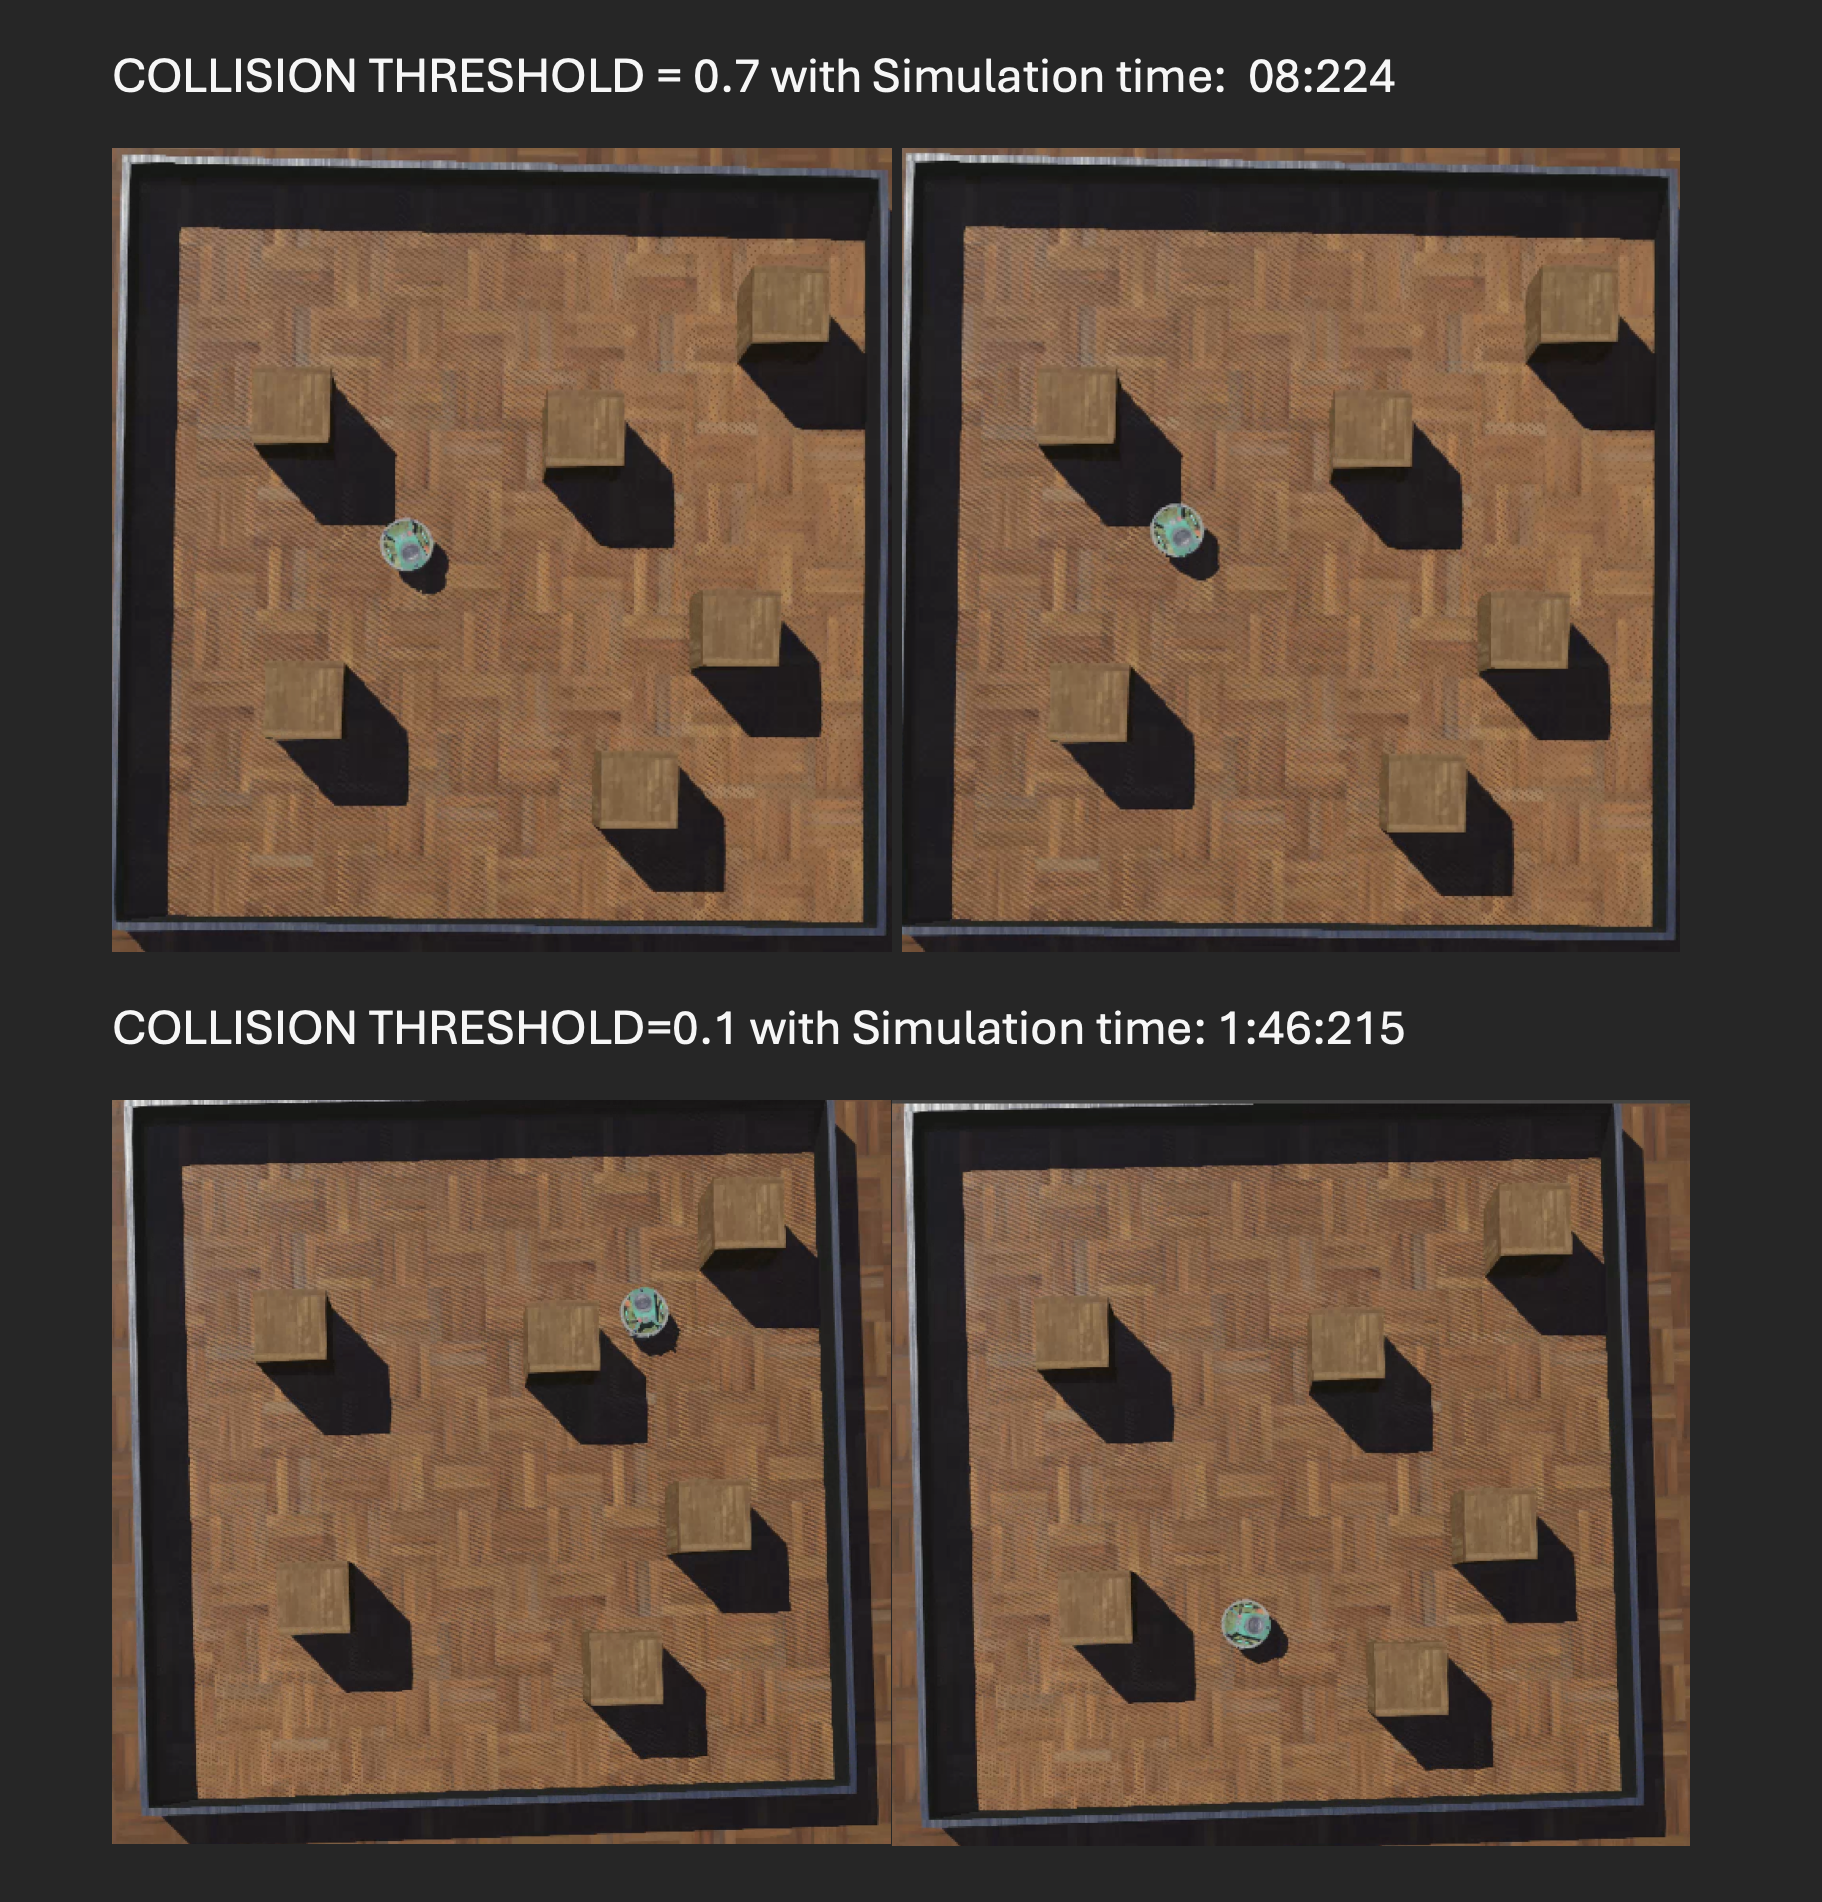
\includegraphics[scale=.25]{deadreckoningError.png}
\end{center}

In the image above, we see that the shorter the simulation runs the more closely the final path matches the replayed path.  And the longer the simulation runs, the more inaccurate the replayed path is.  We believe this is because when replaying the velocities and durations we are essentially doing \textbf{DEAD RECKONING}.  In other words, we are integrating our velocities and durations in the hope that they lead to our final goal.  However, small errors in the replayed durations and velocities accumulate over the course of the simulation and lead to more and more drift from our final goal. 

\end{framed}

\section{Dynamics and Control}

\begin{framed}
\subsection{ Part A - 2 Points}
\label{sec:DynAndCtrl}
\end{framed}


\end{document}